\documentclass[letterpaper,12pt]{article}\usepackage[]{graphicx}\usepackage[]{color}
%% maxwidth is the original width if it is less than linewidth
%% otherwise use linewidth (to make sure the graphics do not exceed the margin)
\makeatletter
\def\maxwidth{ %
  \ifdim\Gin@nat@width>\linewidth
    \linewidth
  \else
    \Gin@nat@width
  \fi
}
\makeatother

\definecolor{fgcolor}{rgb}{0.345, 0.345, 0.345}
\newcommand{\hlnum}[1]{\textcolor[rgb]{0.686,0.059,0.569}{#1}}%
\newcommand{\hlstr}[1]{\textcolor[rgb]{0.192,0.494,0.8}{#1}}%
\newcommand{\hlcom}[1]{\textcolor[rgb]{0.678,0.584,0.686}{\textit{#1}}}%
\newcommand{\hlopt}[1]{\textcolor[rgb]{0,0,0}{#1}}%
\newcommand{\hlstd}[1]{\textcolor[rgb]{0.345,0.345,0.345}{#1}}%
\newcommand{\hlkwa}[1]{\textcolor[rgb]{0.161,0.373,0.58}{\textbf{#1}}}%
\newcommand{\hlkwb}[1]{\textcolor[rgb]{0.69,0.353,0.396}{#1}}%
\newcommand{\hlkwc}[1]{\textcolor[rgb]{0.333,0.667,0.333}{#1}}%
\newcommand{\hlkwd}[1]{\textcolor[rgb]{0.737,0.353,0.396}{\textbf{#1}}}%
\let\hlipl\hlkwb

\usepackage{framed}
\makeatletter
\newenvironment{kframe}{%
 \def\at@end@of@kframe{}%
 \ifinner\ifhmode%
  \def\at@end@of@kframe{\end{minipage}}%
  \begin{minipage}{\columnwidth}%
 \fi\fi%
 \def\FrameCommand##1{\hskip\@totalleftmargin \hskip-\fboxsep
 \colorbox{shadecolor}{##1}\hskip-\fboxsep
     % There is no \\@totalrightmargin, so:
     \hskip-\linewidth \hskip-\@totalleftmargin \hskip\columnwidth}%
 \MakeFramed {\advance\hsize-\width
   \@totalleftmargin\z@ \linewidth\hsize
   \@setminipage}}%
 {\par\unskip\endMakeFramed%
 \at@end@of@kframe}
\makeatother

\definecolor{shadecolor}{rgb}{.97, .97, .97}
\definecolor{messagecolor}{rgb}{0, 0, 0}
\definecolor{warningcolor}{rgb}{1, 0, 1}
\definecolor{errorcolor}{rgb}{1, 0, 0}
\newenvironment{knitrout}{}{} % an empty environment to be redefined in TeX

\usepackage{alltt}
\usepackage[top=1in,bottom=1in,left=1in,right=1in]{geometry}
\usepackage{setspace}
\usepackage[colorlinks=true,urlcolor=blue,citecolor=blue,linkcolor=blue]{hyperref}
\usepackage{indentfirst}
\usepackage{multirow}
\usepackage{booktabs}
\usepackage[final]{animate}
\usepackage{graphicx}
\usepackage{verbatim}
\usepackage{rotating}
\usepackage{tabularx}
\usepackage{array}
\usepackage{subfig} 
\usepackage[noae]{Sweave}
\usepackage{cleveref}
\usepackage[figureposition=bottom]{caption}
\usepackage{paralist}
\usepackage{acronym}
\usepackage{outlines}
\usepackage{pdflscape}

% knitr options


% housekeeping


\linespread{1}
\IfFileExists{upquote.sty}{\usepackage{upquote}}{}
\begin{document}
\title{Analysis of 16S microbial sequencing data from a Southern Califoria WWTP discharge fields}
\maketitle

\begin{knitrout}
\definecolor{shadecolor}{rgb}{0.969, 0.969, 0.969}\color{fgcolor}

{\centering 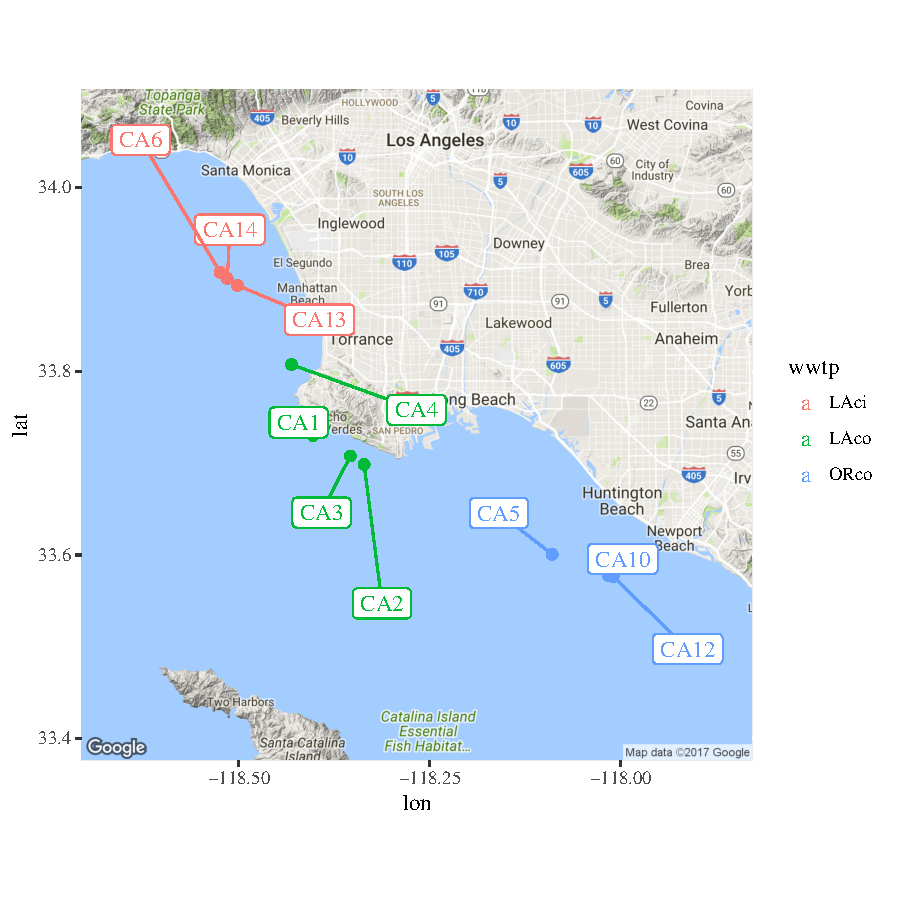
\includegraphics[width=\maxwidth]{figs/unnamed-chunk-2-1} 
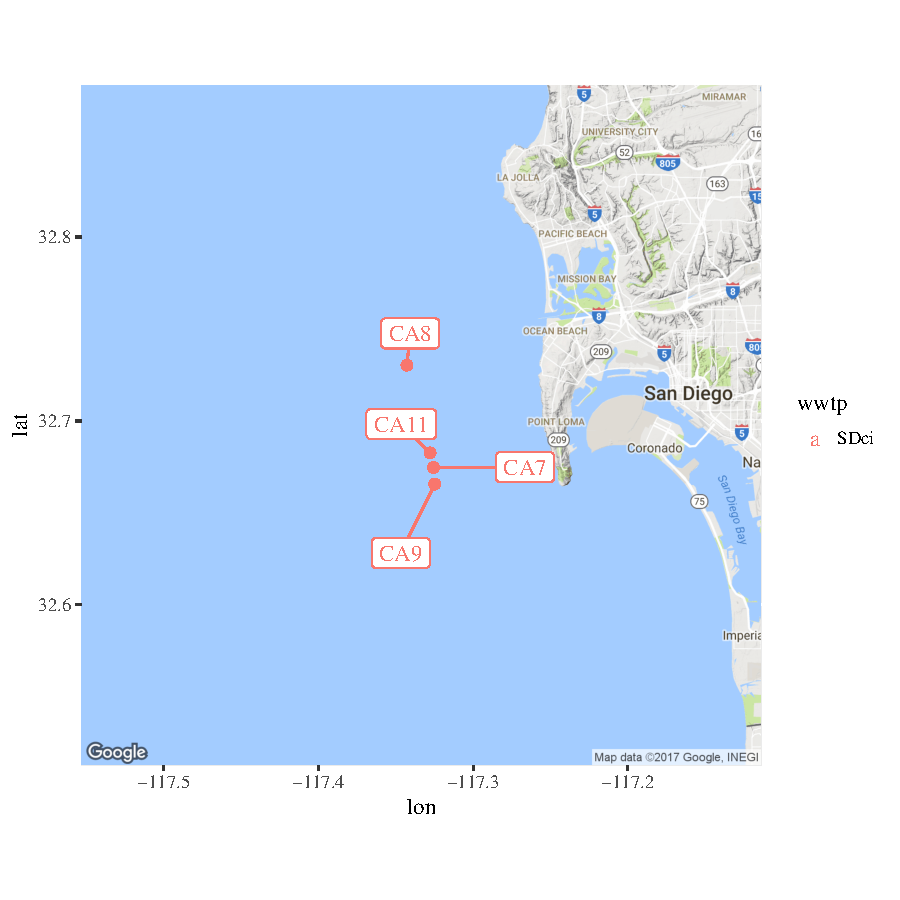
\includegraphics[width=\maxwidth]{figs/unnamed-chunk-2-2} 

}



\end{knitrout}

\begin{knitrout}
\definecolor{shadecolor}{rgb}{0.969, 0.969, 0.969}\color{fgcolor}\begin{kframe}
\begin{alltt}
\hlkwd{load}\hlstd{(}\hlkwc{file} \hlstd{=} \hlstr{'data/abudat.RData'}\hlstd{)}
\hlkwd{lapply}\hlstd{(abudat, head)}
\end{alltt}
\begin{verbatim}
## $DOMAIN
## # A tibble: 6 x 5
## # Groups:   site, wwtp, cont [6]
##    domain  site  wwtp  cont abund
##     <chr> <chr> <chr> <chr> <dbl>
## 1 Archaea   CA1  LACO   int   148
## 2 Archaea  CA10  ORCO   int    50
## 3 Archaea  CA11  SDCI   int    70
## 4 Archaea  CA12  ORCO   clo   104
## 5 Archaea  CA13  LACI   far    96
## 6 Archaea  CA14  LACI   int   139
## 
## $PHYLUM
## # A tibble: 6 x 6
## # Groups:   site, wwtp, cont [6]
##   phylum  site  wwtp  cont abund   domain
##    <chr> <chr> <chr> <chr> <dbl>    <chr>
## 1    AC1   CA1  LACO   int     2 Bacteria
## 2    AC1  CA10  ORCO   int     0 Bacteria
## 3    AC1  CA11  SDCI   int     0 Bacteria
## 4    AC1  CA12  ORCO   clo     0 Bacteria
## 5    AC1  CA13  LACI   far     0 Bacteria
## 6    AC1  CA14  LACI   int     0 Bacteria
## 
## $CLASS
## # A tibble: 6 x 7
## # Groups:   site, wwtp, cont [6]
##            class  site  wwtp  cont abund   domain         phylum
##            <chr> <chr> <chr> <chr> <dbl>    <chr>          <chr>
## 1 028H05-P-BN-P5   CA1  LACO   int     0 Bacteria Planctomycetes
## 2 028H05-P-BN-P5  CA10  ORCO   int     0 Bacteria Planctomycetes
## 3 028H05-P-BN-P5  CA11  SDCI   int     0 Bacteria Planctomycetes
## 4 028H05-P-BN-P5  CA12  ORCO   clo     0 Bacteria Planctomycetes
## 5 028H05-P-BN-P5  CA13  LACI   far     0 Bacteria Planctomycetes
## 6 028H05-P-BN-P5  CA14  LACI   int     0 Bacteria Planctomycetes
## 
## $ORDER
## # A tibble: 6 x 8
## # Groups:   site, wwtp, cont [6]
##               order  site  wwtp  cont abund   domain         phylum
##               <chr> <chr> <chr> <chr> <dbl>    <chr>          <chr>
## 1 028H05-P-BN-P5_or   CA1  LACO   int     0 Bacteria Planctomycetes
## 2 028H05-P-BN-P5_or  CA10  ORCO   int     0 Bacteria Planctomycetes
## 3 028H05-P-BN-P5_or  CA11  SDCI   int     0 Bacteria Planctomycetes
## 4 028H05-P-BN-P5_or  CA12  ORCO   clo     0 Bacteria Planctomycetes
## 5 028H05-P-BN-P5_or  CA13  LACI   far     0 Bacteria Planctomycetes
## 6 028H05-P-BN-P5_or  CA14  LACI   int     0 Bacteria Planctomycetes
## # ... with 1 more variables: class <chr>
## 
## $FAMILY
## # A tibble: 6 x 9
## # Groups:   site, wwtp, cont [6]
##    family  site  wwtp  cont abund   domain          phylum          class
##     <chr> <chr> <chr> <chr> <dbl>    <chr>           <chr>          <chr>
## 1 01D2Z36   CA1  LACO   int     0 Bacteria Verrucomicrobia Spartobacteria
## 2 01D2Z36  CA10  ORCO   int     0 Bacteria Verrucomicrobia Spartobacteria
## 3 01D2Z36  CA11  SDCI   int     0 Bacteria Verrucomicrobia Spartobacteria
## 4 01D2Z36  CA12  ORCO   clo     0 Bacteria Verrucomicrobia Spartobacteria
## 5 01D2Z36  CA13  LACI   far     0 Bacteria Verrucomicrobia Spartobacteria
## 6 01D2Z36  CA14  LACI   int     1 Bacteria Verrucomicrobia Spartobacteria
## # ... with 1 more variables: order <chr>
## 
## $GENUS
## # A tibble: 6 x 10
## # Groups:   site, wwtp, cont [6]
##        genus  site  wwtp  cont abund   domain          phylum
##        <chr> <chr> <chr> <chr> <dbl>    <chr>           <chr>
## 1 01D2Z36_ge   CA1  LACO   int     0 Bacteria Verrucomicrobia
## 2 01D2Z36_ge  CA10  ORCO   int     0 Bacteria Verrucomicrobia
## 3 01D2Z36_ge  CA11  SDCI   int     0 Bacteria Verrucomicrobia
## 4 01D2Z36_ge  CA12  ORCO   clo     0 Bacteria Verrucomicrobia
## 5 01D2Z36_ge  CA13  LACI   far     0 Bacteria Verrucomicrobia
## 6 01D2Z36_ge  CA14  LACI   int     1 Bacteria Verrucomicrobia
## # ... with 3 more variables: class <chr>, order <chr>, family <chr>
## 
## $SPECIES
## # A tibble: 6 x 11
## # Groups:   site, wwtp, cont [6]
##    species  site  wwtp  cont abund   domain     phylum   class      order
##      <chr> <chr> <chr> <chr> <dbl>    <chr>      <chr>   <chr>      <chr>
## 1 Otu00001   CA1  LACO   int  4993 Bacteria Firmicutes Bacilli Bacillales
## 2 Otu00001  CA10  ORCO   int  7001 Bacteria Firmicutes Bacilli Bacillales
## 3 Otu00001  CA11  SDCI   int  2573 Bacteria Firmicutes Bacilli Bacillales
## 4 Otu00001  CA12  ORCO   clo   703 Bacteria Firmicutes Bacilli Bacillales
## 5 Otu00001  CA13  LACI   far   842 Bacteria Firmicutes Bacilli Bacillales
## 6 Otu00001  CA14  LACI   int  1578 Bacteria Firmicutes Bacilli Bacillales
## # ... with 2 more variables: family <chr>, genus <chr>
\end{verbatim}
\end{kframe}
\end{knitrout}

\section{Community structure}
 
\begin{knitrout}
\definecolor{shadecolor}{rgb}{0.969, 0.969, 0.969}\color{fgcolor}\begin{figure}[!ht]

{\centering 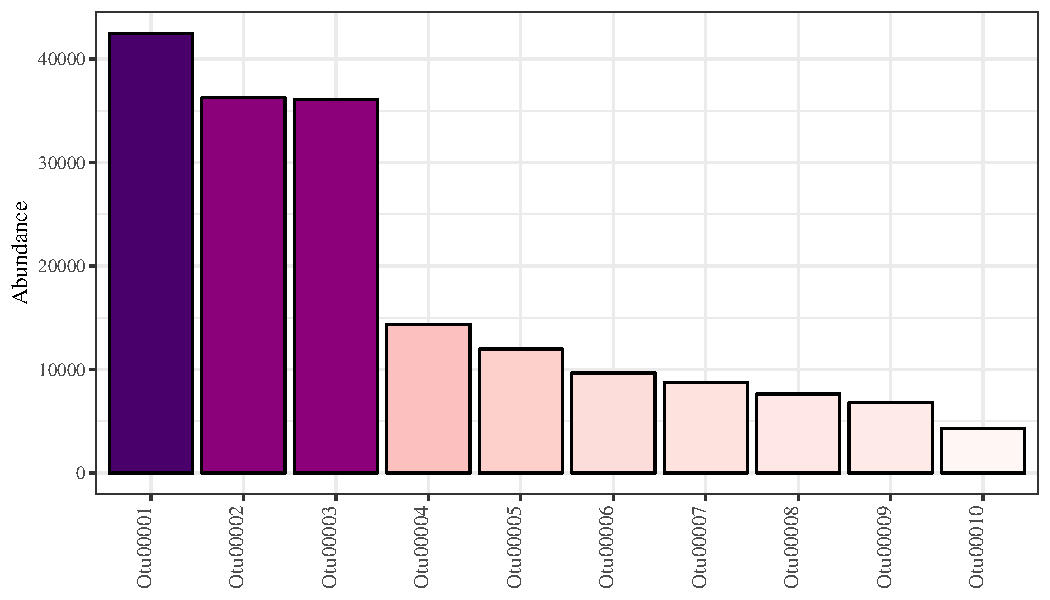
\includegraphics[width=0.8\textwidth]{figs/abundall-1} 

}

\caption[Top fifty most abundant species across all study sites]{Top fifty most abundant species across all study sites.}\label{fig:abundall}
\end{figure}


\end{knitrout}

\begin{knitrout}
\definecolor{shadecolor}{rgb}{0.969, 0.969, 0.969}\color{fgcolor}\begin{figure}[!ht]

{\centering 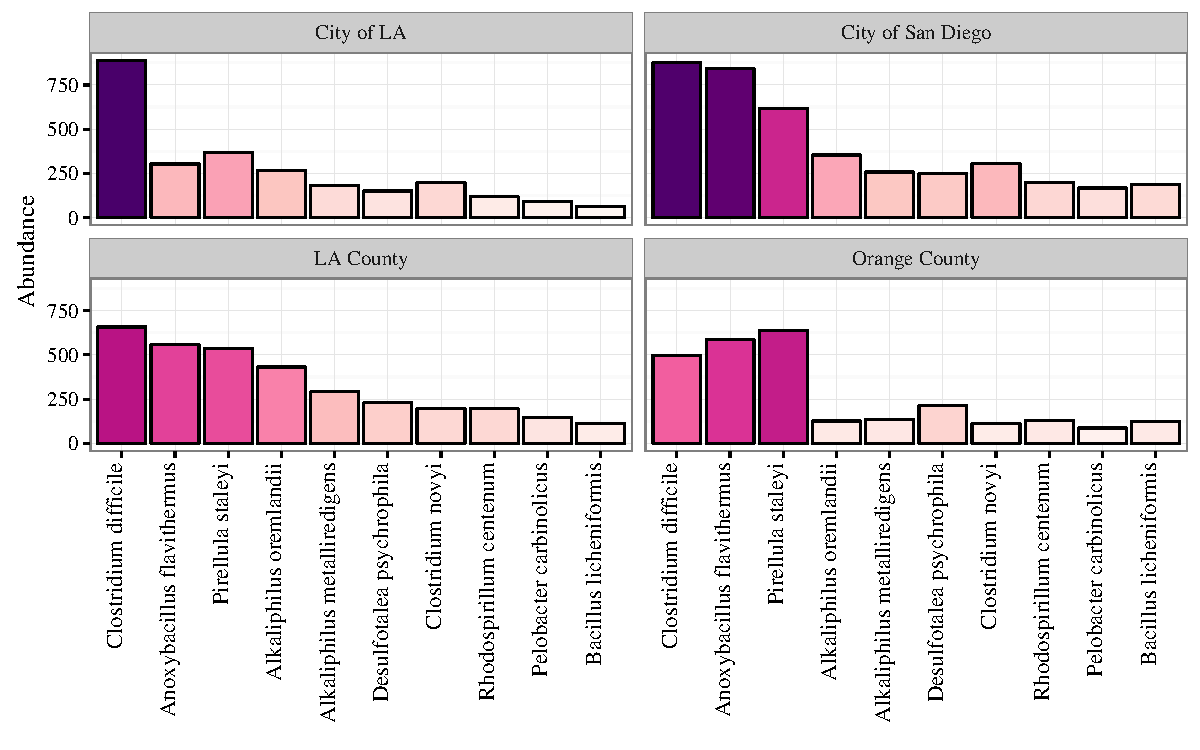
\includegraphics[width=0.8\textwidth]{figs/abundmuni-1} 

}

\caption{Species abundances by municipal locations using the top fifty most abundant across all study sites in \cref{fig:abundall}.}\label{fig:abundmuni}
\end{figure}


\end{knitrout}
\clearpage

\begin{knitrout}
\definecolor{shadecolor}{rgb}{0.969, 0.969, 0.969}\color{fgcolor}\begin{figure}[!ht]

{\centering 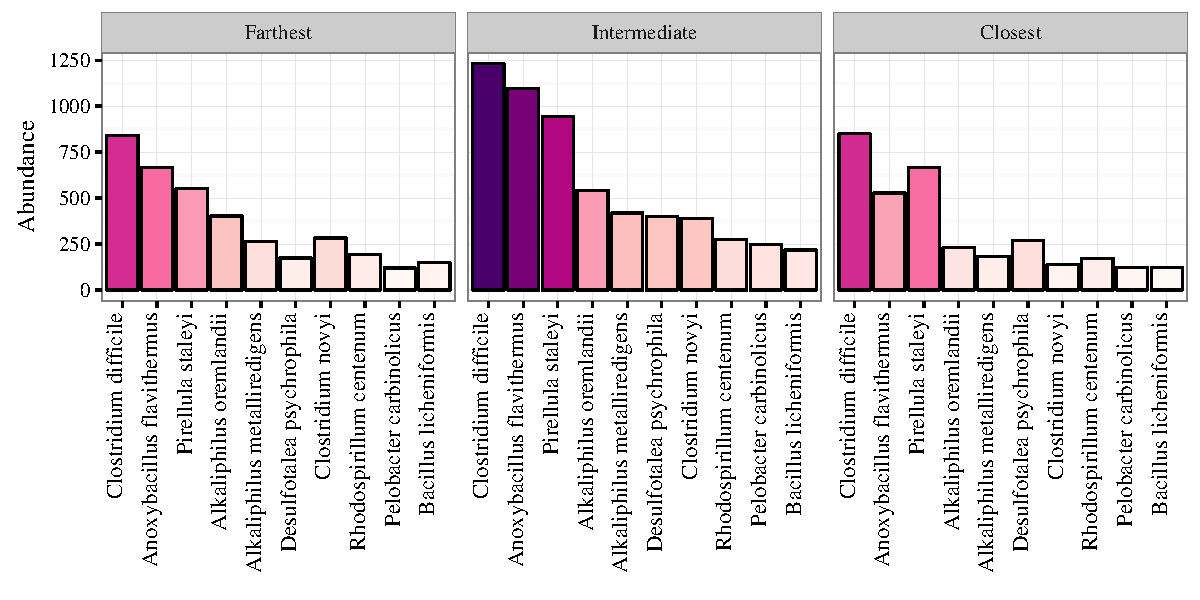
\includegraphics[width=0.8\textwidth]{figs/abundcont-1} 

}

\caption{Species abundances by distance from pipe for the top fifty most abundant across all study sites in \cref{fig:abundall}.  Treatments are based on relative distances from an outflow pipe (farthest, intermediate, closest) for each municipality.}\label{fig:abundcont}
\end{figure}


\end{knitrout}
\clearpage

\begin{landscape}
\centering\vspace*{\fill}
\begin{knitrout}
\definecolor{shadecolor}{rgb}{0.969, 0.969, 0.969}\color{fgcolor}\begin{figure}[!ht]

{\centering 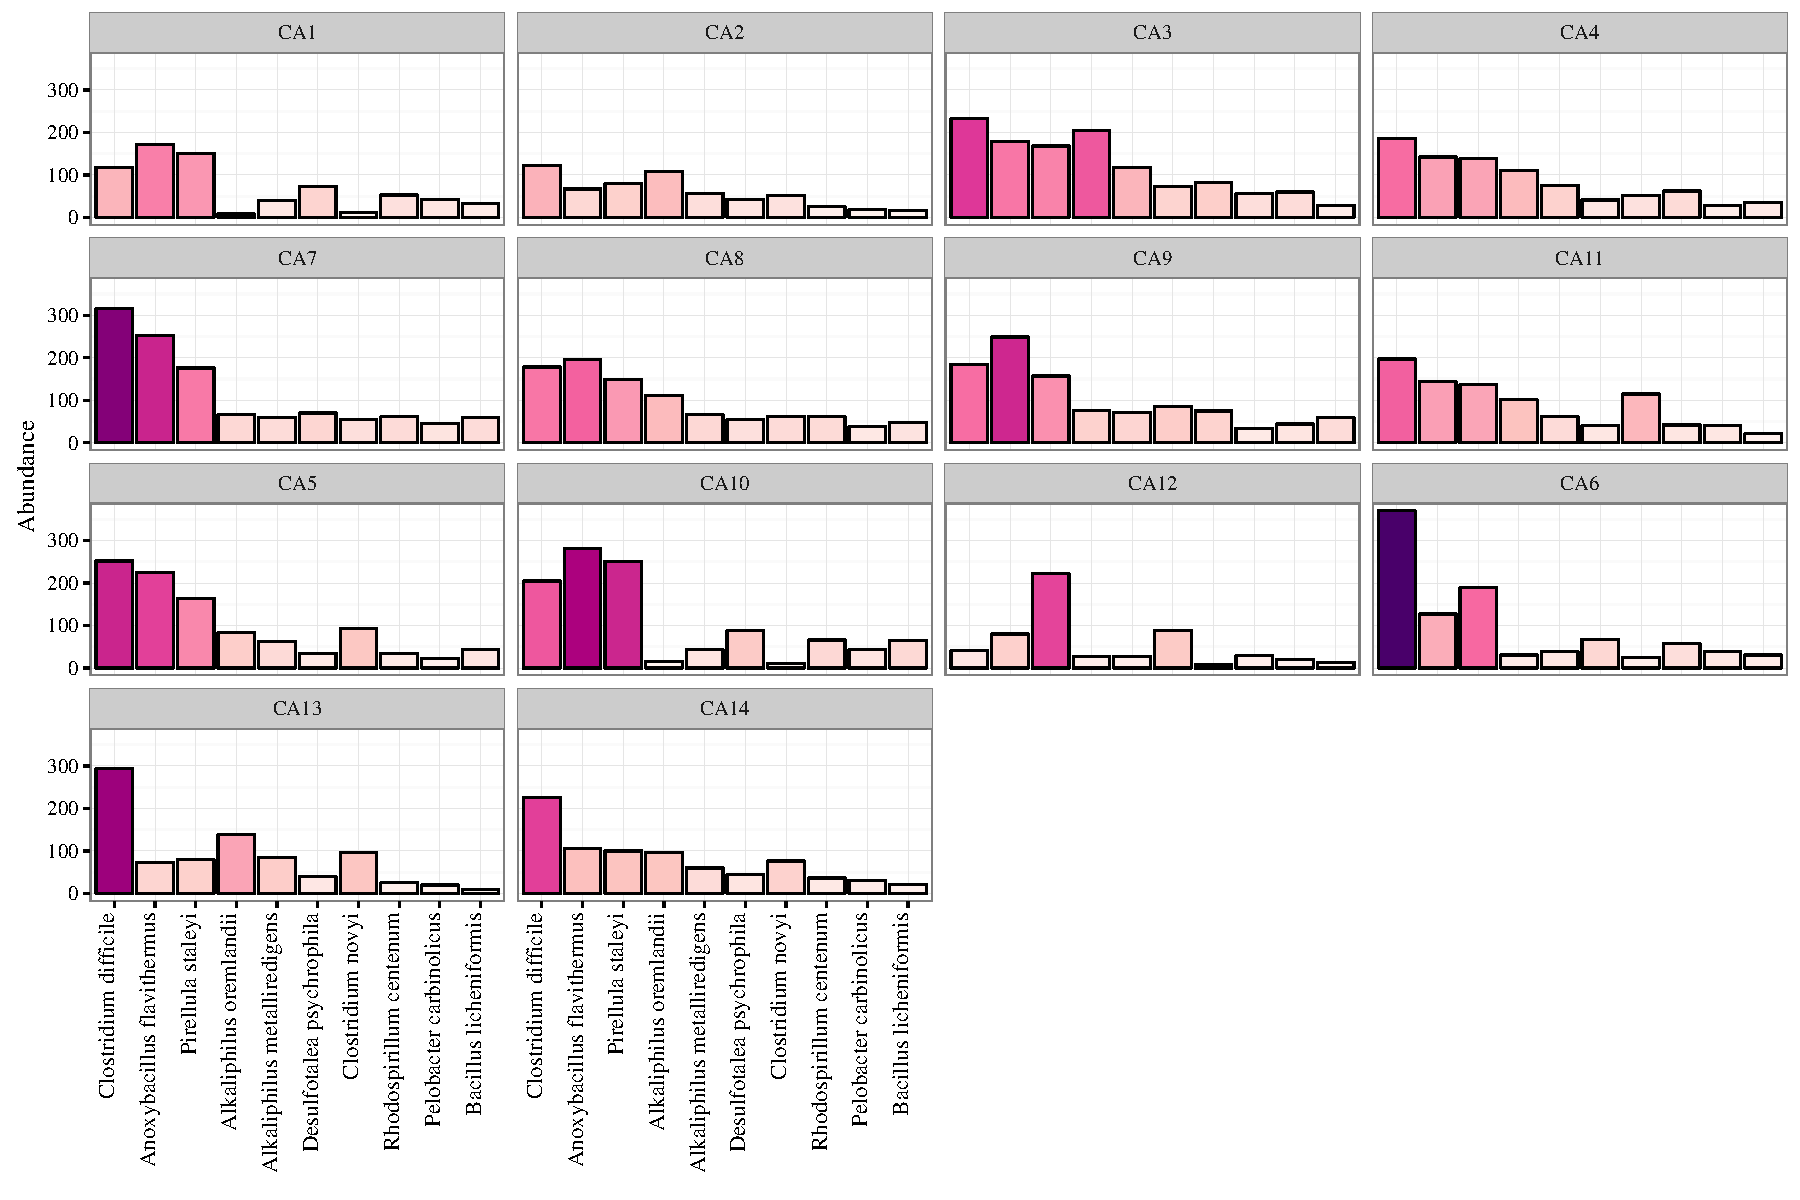
\includegraphics[width=1.1\textwidth]{figs/abundsite-1} 

}

\caption{Species abundances by sites using the top fifty most abundant across all study sites in \cref{fig:abundall}.}\label{fig:abundsite}
\end{figure}


\end{knitrout}
\end{landscape}
\clearpage

\subsection{Multivariate analyses with archaea}

\begin{knitrout}
\definecolor{shadecolor}{rgb}{0.969, 0.969, 0.969}\color{fgcolor}\begin{figure}[!ht]

{\centering 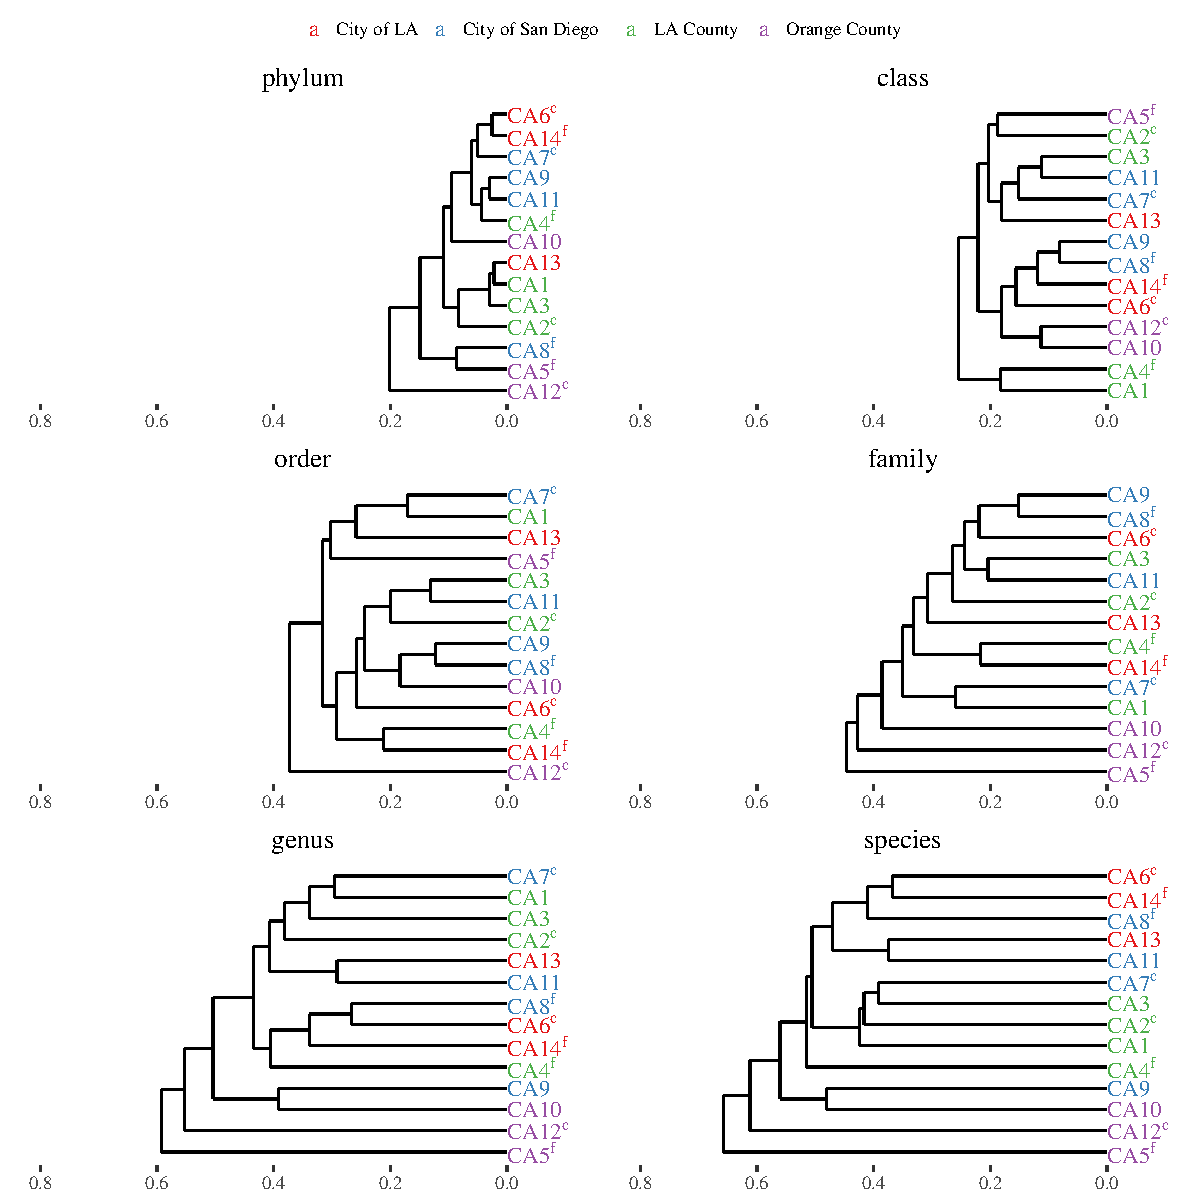
\includegraphics[width=\textwidth]{figs/clust1_arch-1} 

}

\caption[Site clusters of archaea by taxonomic resolution]{Site clusters of archaea by taxonomic resolution.  Colors indicate municipality and superscripts indicate distance categories from an outflow pipe at each site (`f' is farthest, `c' is closest, none is intermediate).  Clustering was based on a Bray-Curtis dissimilarity matrix of abundance data and sorting using the unweighted pair group method.}\label{fig:clust1_arch}
\end{figure}


\end{knitrout}

\begin{knitrout}
\definecolor{shadecolor}{rgb}{0.969, 0.969, 0.969}\color{fgcolor}\begin{figure}[!ht]

{\centering 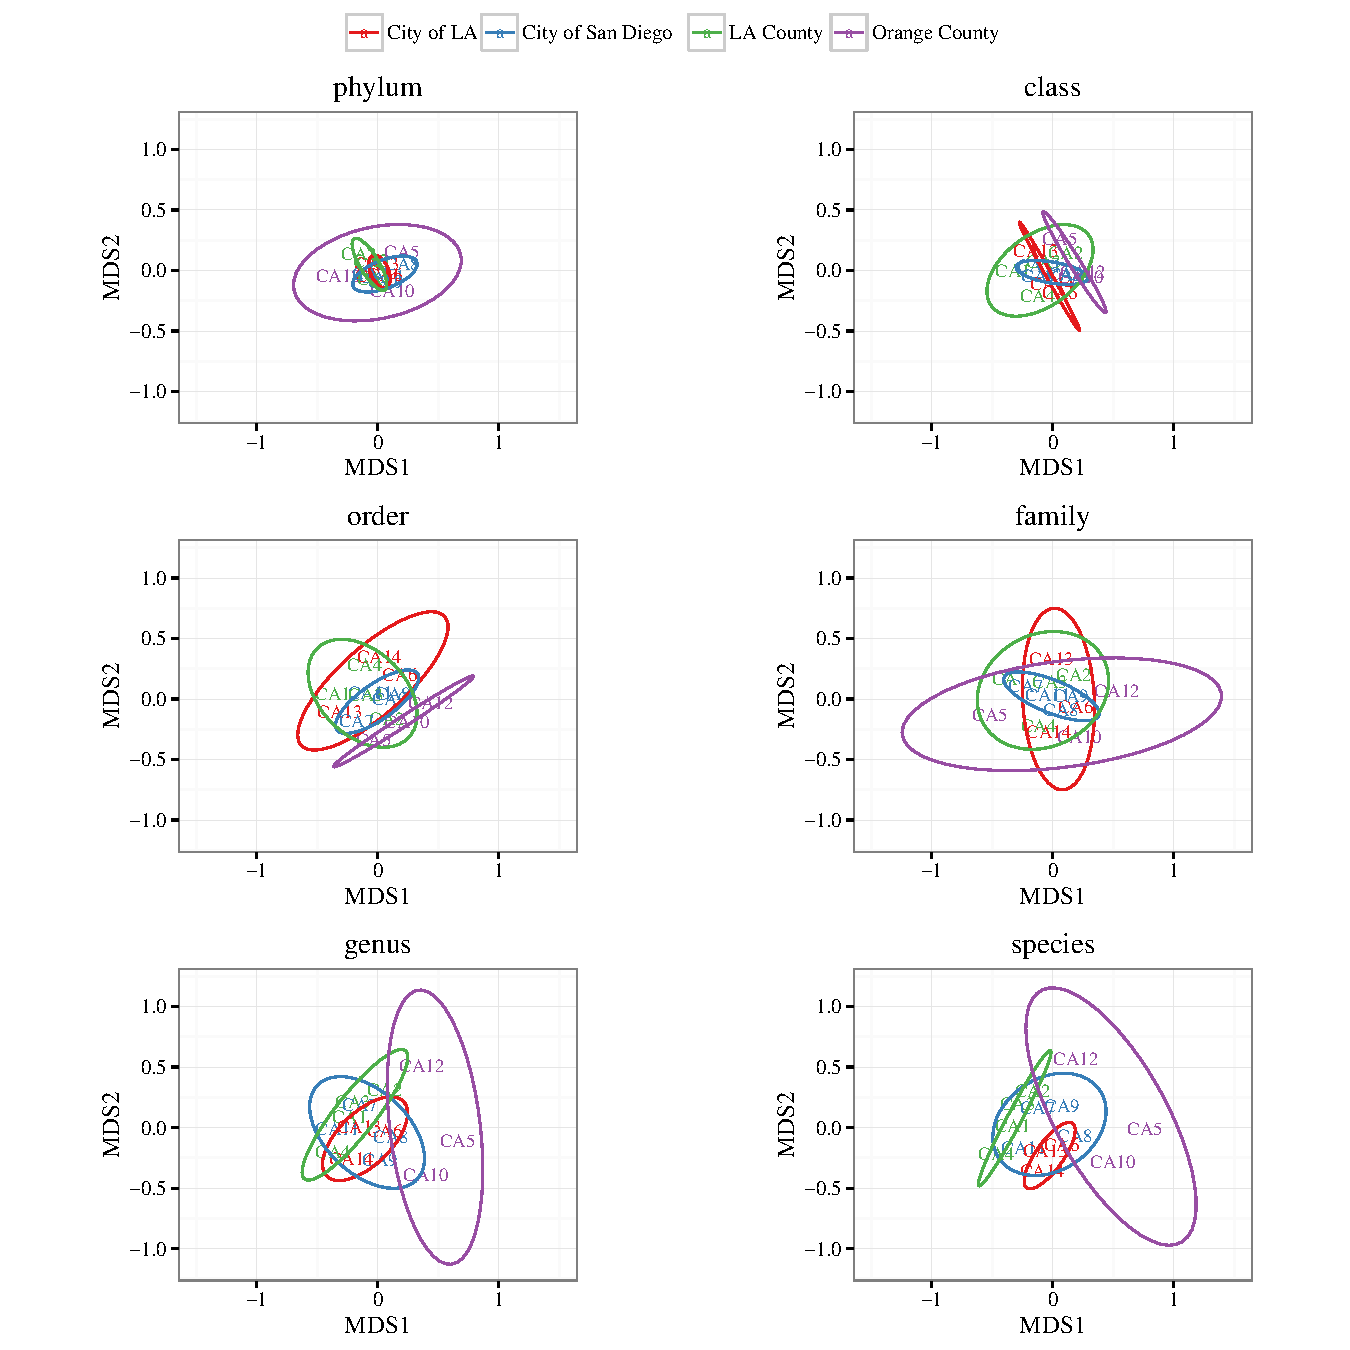
\includegraphics[width=\textwidth]{figs/ord1_arch-1} 

}

\caption{Site ordinations of archaea by taxonomic resolution.  Colors indicate municipality with ellipses showing 95\% bivariate confidence intervals.  Ordinations were created using Nonmetric Multidimensional scaling with several random starts to find a stable solution of the configuration.  A Bray-Curtis dissimilarity matrix was used as a measure of differences between sites. The ordination is the same as in \cref{fig:ord2_arch} but with different group categories in the plot.}\label{fig:ord1_arch}
\end{figure}


\end{knitrout}

\begin{knitrout}
\definecolor{shadecolor}{rgb}{0.969, 0.969, 0.969}\color{fgcolor}\begin{figure}[!ht]

{\centering 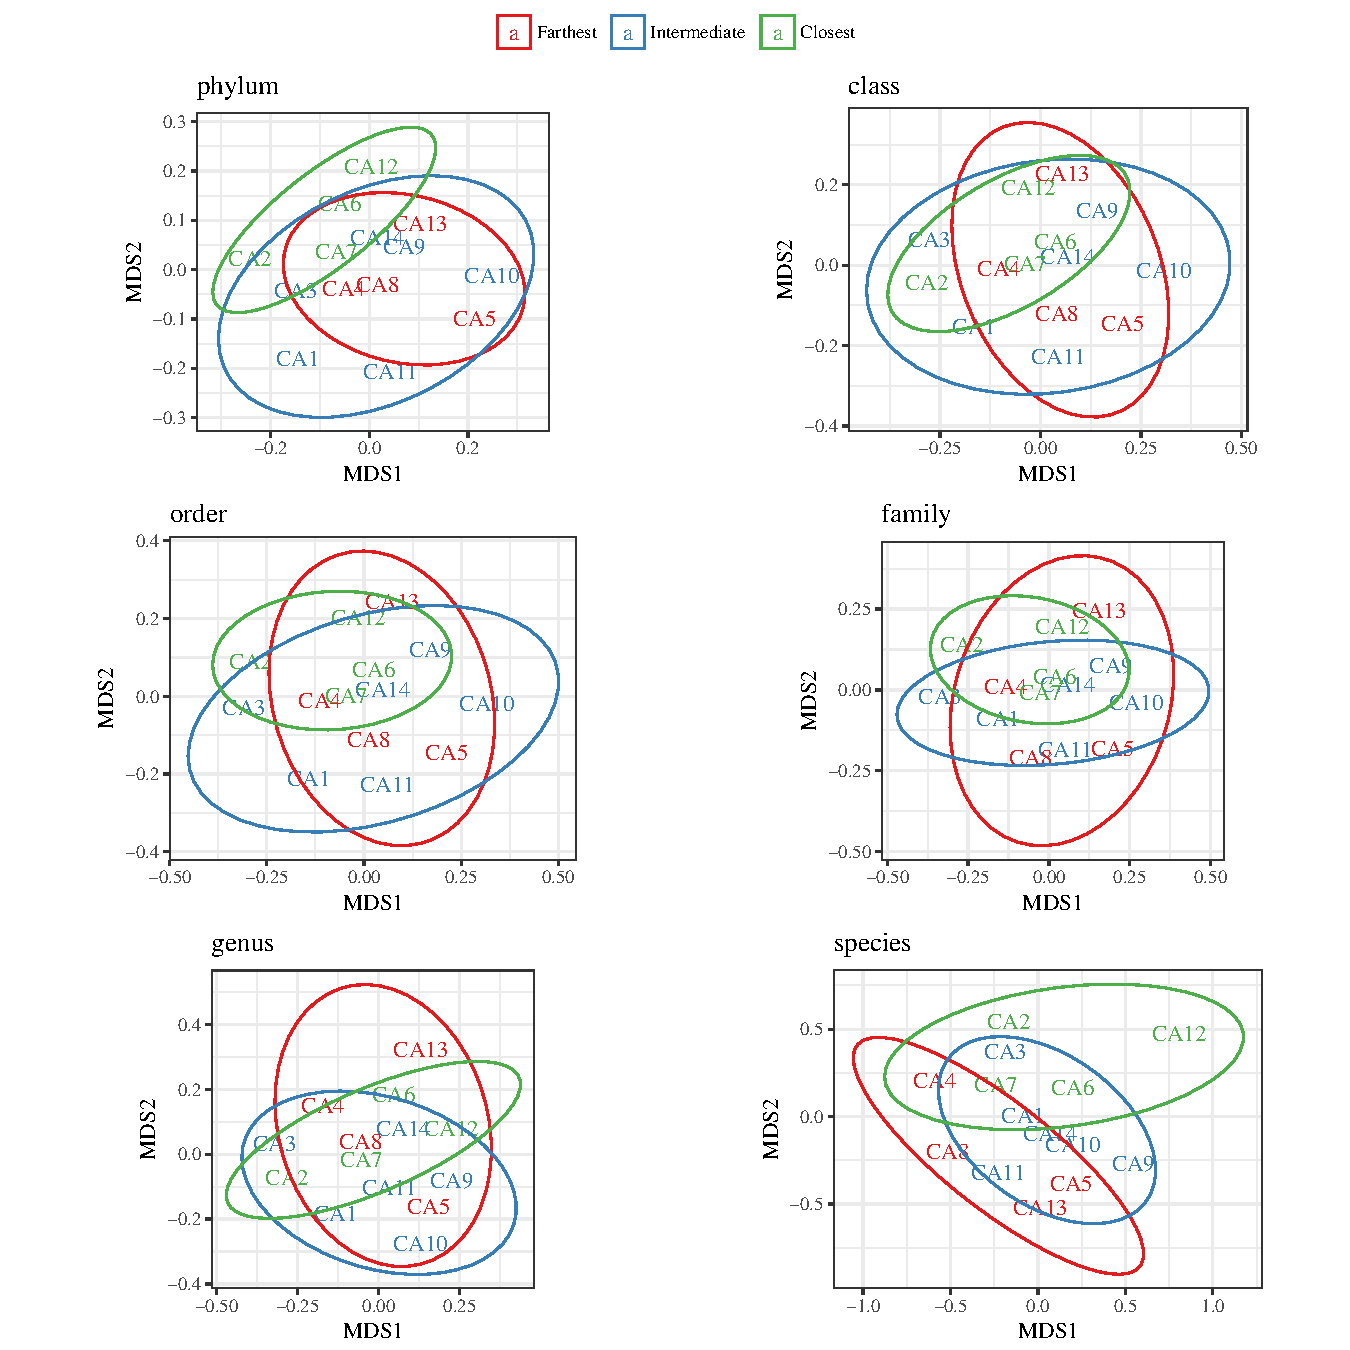
\includegraphics[width=1.05\textwidth]{figs/ord2_arch-1} 

}

\caption{Site ordinations of archaea by taxonomic resolution.  Colors indicate approximate distance from pipe with ellipses showing 95\% bivariate confidence intervals. Ordinations were created using Nonmetric Multidimensional scaling with several random starts to find a stable solution of the configuration.  A Bray-Curtis dissimilarity matrix was used as a measure of differences between sites. The ordination is the same as in \cref{fig:ord1_arch} but with different group categories in the plot.}\label{fig:ord2_arch}
\end{figure}


\end{knitrout}
\clearpage

%latex.default(taba, file = "", rowlabel = "Location grouping",     caption = cap.val, caption.loc = "top", rgroup = c("Municipality",         "Pipe location", "Site"), n.rgroup = c(4, 3, 14), rowname = rows,     label = "tab:alpha_arch")%
\begin{table}[!tbp]
\caption{Alpha diversity of archaea by municipality, distance from outflow, and sites for each taxonomic level.  Original data were taxanomic abundance aggregated by each grouping.  Alpha was was based on methods in Fisher et al. (1943) that measure diversity as a function of richness and abundance at a site.\label{tab:alpha_arch}} 
\begin{center}
\begin{tabular}{lllllll}
\hline\hline
\multicolumn{1}{l}{Location grouping}&\multicolumn{1}{c}{Phylum}&\multicolumn{1}{c}{Class}&\multicolumn{1}{c}{Order}&\multicolumn{1}{c}{Family}&\multicolumn{1}{c}{Genus}&\multicolumn{1}{c}{Species}\tabularnewline
\hline
{\bfseries Municipality}&&&&&&\tabularnewline
~~City of LA&1.83&2.77&3.02&3.80&4.62& 70.34\tabularnewline
~~City of San Diego&1.78&2.70&2.70&3.69&3.95&135.86\tabularnewline
~~LA County&2.07&3.16&3.63&4.10&4.85& 80.58\tabularnewline
~~Orange County&1.65&2.47&2.47&3.06&3.37& 88.71\tabularnewline
\hline
{\bfseries Pipe location}&&&&&&\tabularnewline
~~Farthest&2.06&3.02&3.28&4.34&5.19&109.98\tabularnewline
~~Intermediate&2.11&3.00&3.47&3.95&4.70& 88.42\tabularnewline
~~Closest&1.63&2.44&2.65&3.31&4.00&127.81\tabularnewline
\hline
{\bfseries Site}&&&&&&\tabularnewline
~~CA1&2.11&2.75&2.75&2.75&2.75& 23.76\tabularnewline
~~CA2&2.00&2.79&3.07&3.35&3.64& 46.23\tabularnewline
~~CA3&2.19&3.58&3.96&3.96&3.96& 27.14\tabularnewline
~~CA4&1.67&2.33&2.33&2.68&3.44& 44.31\tabularnewline
~~CA7&1.49&2.35&2.35&2.66&2.98& 86.56\tabularnewline
~~CA8&1.22&1.75&1.75&2.33&2.33& 53.49\tabularnewline
~~CA9&1.50&2.59&2.59&3.00&3.44& 29.57\tabularnewline
~~CA11&3.19&3.67&3.67&4.17&4.17& 47.43\tabularnewline
~~CA5&2.10&3.01&3.01&3.51&3.51& 45.68\tabularnewline
~~CA10&1.78&2.69&2.69&2.69&2.69& 23.95\tabularnewline
~~CA12&1.69&2.73&2.73&3.51&3.92& 59.12\tabularnewline
~~CA6&1.42&2.23&2.23&2.23&3.14& 34.14\tabularnewline
~~CA13&2.43&4.06&4.51&6.00&7.10& 38.20\tabularnewline
~~CA14&1.28&2.15&2.15&2.47&3.15& 30.15\tabularnewline
\hline
\end{tabular}\end{center}
\end{table}
%latex.default(tabb, file = "", rowlabel = "Location grouping",     caption = cap.val, caption.loc = "top", rowname = rows, label = "tab:beta_arch")%
\begin{table}[!tbp]
\caption{Beta diversity of archaea between municipalities, distance categories from outflow, and sites for each taxonomic level.  Original data were taxonomic abundance aggregated by each grouping.  Beta was estimated as total species richness across all categories in each grouping, divided by mean species richness within each category, minus one.\label{tab:beta_arch}} 
\begin{center}
\begin{tabular}{lllllll}
\hline\hline
\multicolumn{1}{l}{Location grouping}&\multicolumn{1}{c}{Phylum}&\multicolumn{1}{c}{Class}&\multicolumn{1}{c}{Order}&\multicolumn{1}{c}{Family}&\multicolumn{1}{c}{Genus}&\multicolumn{1}{c}{Species}\tabularnewline
\hline
Distance from outflow&0.18&0.27&0.35&0.45&0.48&1.39\tabularnewline
Site&0.72&0.86&1.11&1.45&1.67&7.64\tabularnewline
Municipality&0.30&0.36&0.49&0.60&0.69&2.05\tabularnewline
\hline
\end{tabular}\end{center}
\end{table}


\subsection{Multivariate analyses with bacteria}

\begin{knitrout}
\definecolor{shadecolor}{rgb}{0.969, 0.969, 0.969}\color{fgcolor}\begin{figure}[!ht]

{\centering 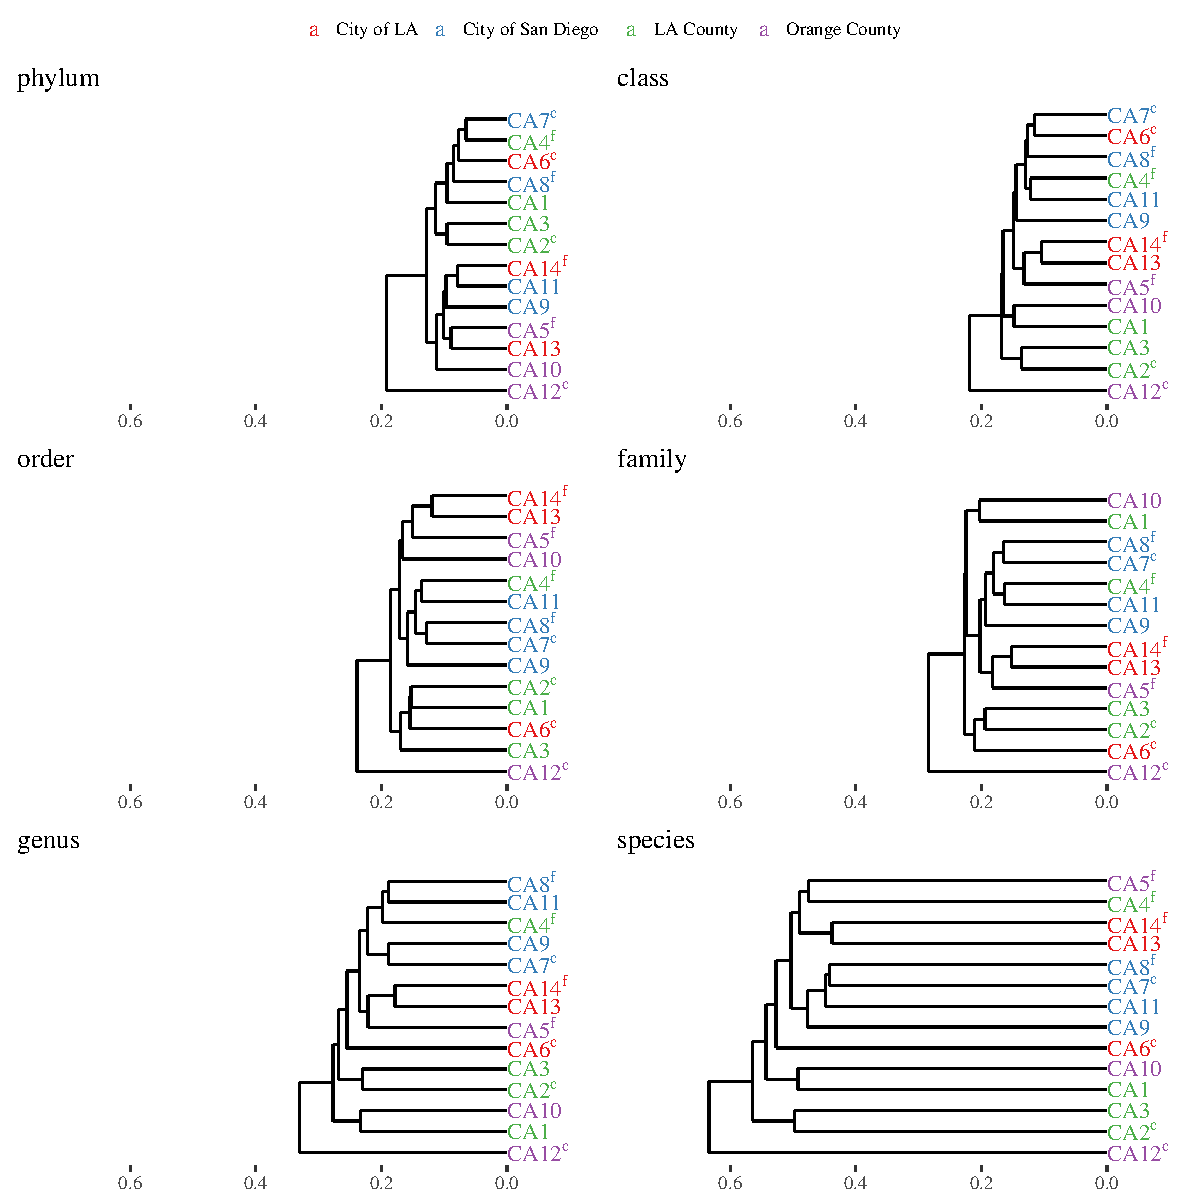
\includegraphics[width=\textwidth]{figs/clust1_bac-1} 

}

\caption[Site clusters of bacteria by taxonomic resolution]{Site clusters of bacteria by taxonomic resolution.  Colors indicate municipality and superscripts indicate distance categories from an outflow pipe at each site (`f' is farthest, `c' is closest, none is intermediate).  Clustering was based on a Bray-Curtis dissimilarity matrix of abundance data and sorting using the unweighted pair group method.}\label{fig:clust1_bac}
\end{figure}


\end{knitrout}

\begin{knitrout}
\definecolor{shadecolor}{rgb}{0.969, 0.969, 0.969}\color{fgcolor}\begin{figure}[!ht]

{\centering 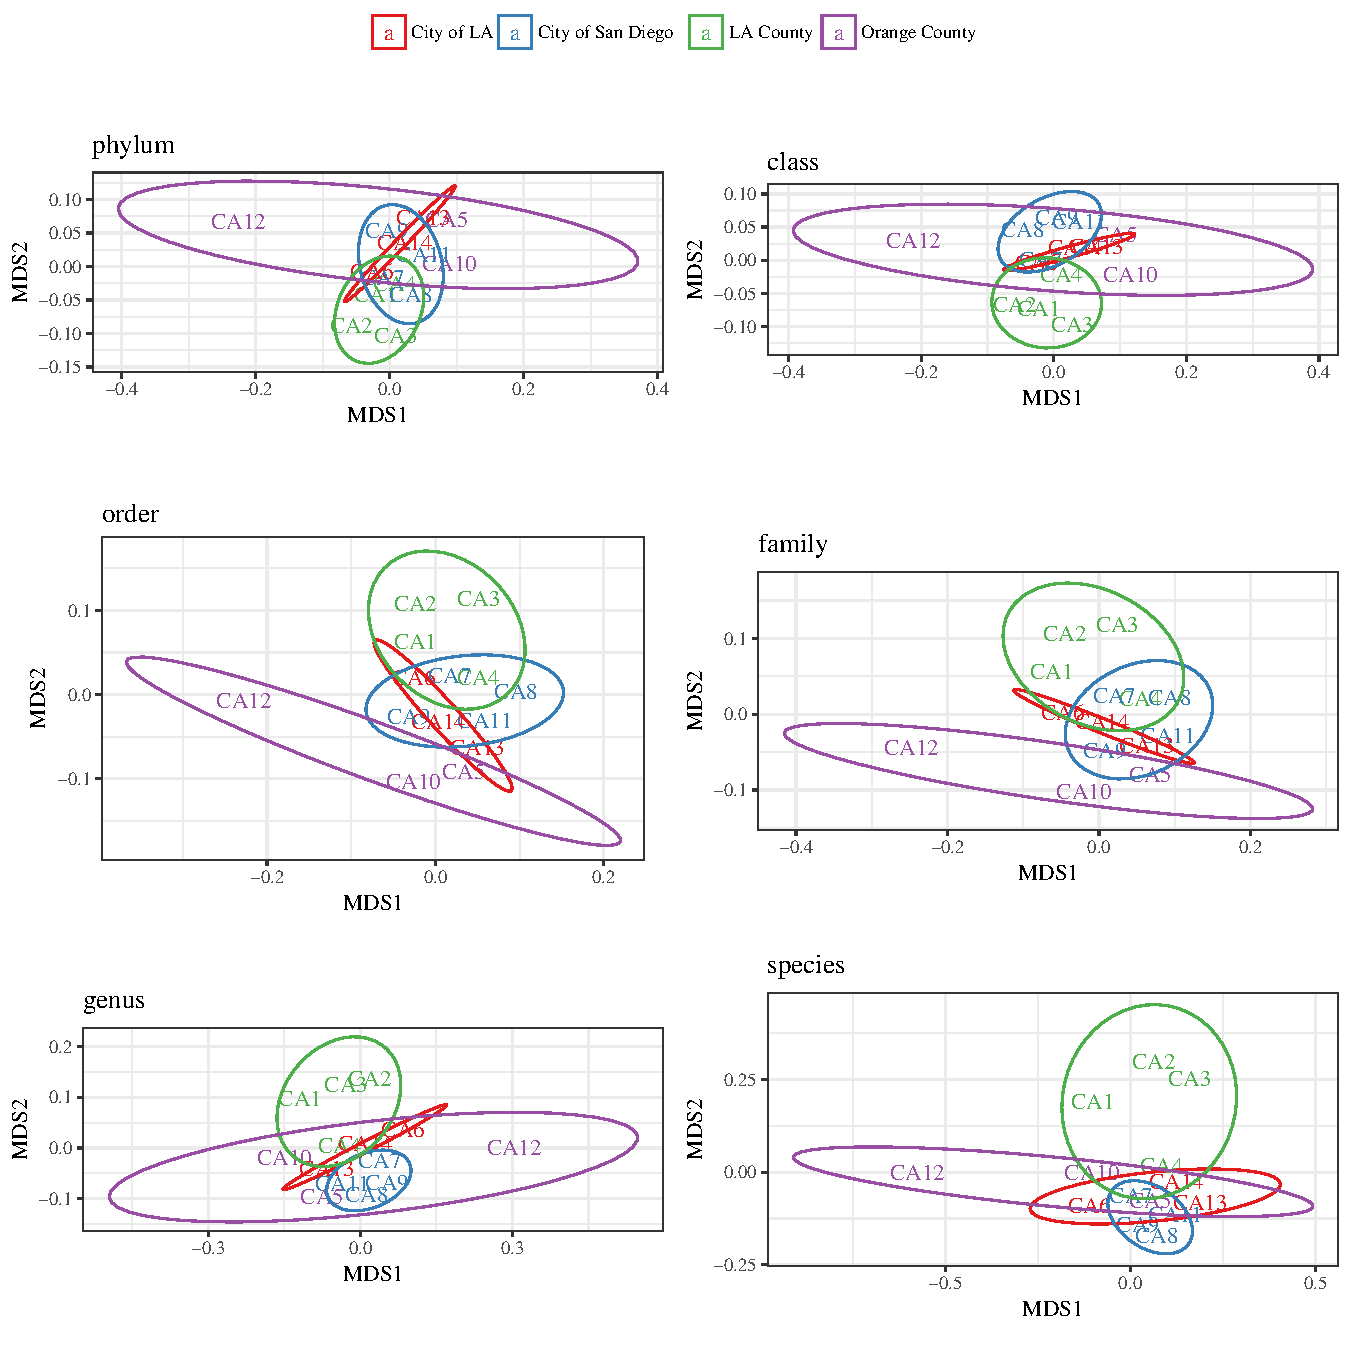
\includegraphics[width=\textwidth]{figs/ord1_bac-1} 

}

\caption{Site ordinations of bacteria by taxonomic resolution.  Colors indicate municipality with ellipses showing 95\% bivariate confidence intervals.  Ordinations were created using Nonmetric Multidimensional scaling with several random starts to find a stable solution of the configuration.  A Bray-Curtis dissimilarity matrix was used as a measure of differences between sites. The ordination is the same as in \cref{fig:ord2_bac} but with different group categories in the plot.}\label{fig:ord1_bac}
\end{figure}


\end{knitrout}

\begin{knitrout}
\definecolor{shadecolor}{rgb}{0.969, 0.969, 0.969}\color{fgcolor}\begin{figure}[!ht]

{\centering 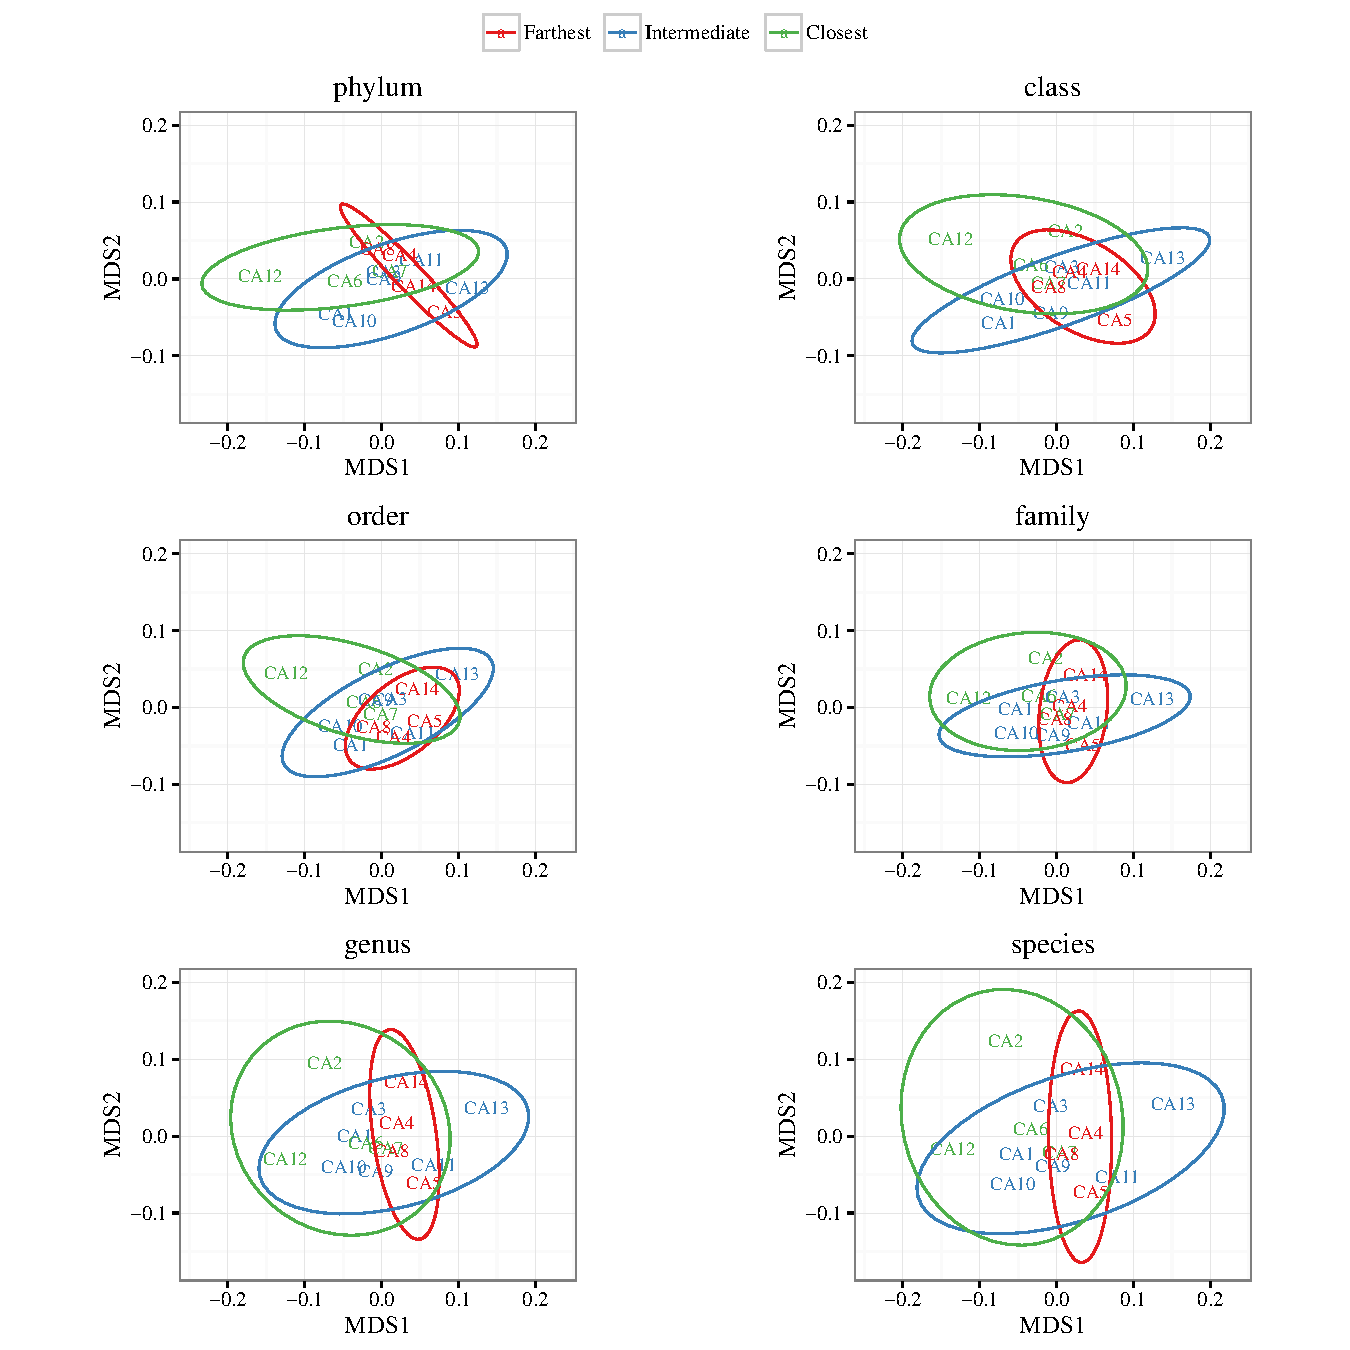
\includegraphics[width=1.05\textwidth]{figs/ord2_bac-1} 

}

\caption{Site ordinations of bacteria by taxonomic resolution.  Colors indicate approximate distance from pipe with ellipses showing 95\% bivariate confidence intervals. Ordinations were created using Nonmetric Multidimensional scaling with several random starts to find a stable solution of the configuration.  A Bray-Curtis dissimilarity matrix was used as a measure of differences between sites. The ordination is the same as in \cref{fig:ord1_bac} but with different group categories in the plot.}\label{fig:ord2_bac}
\end{figure}


\end{knitrout}
\clearpage

%latex.default(taba, file = "", rowlabel = "Location grouping",     caption = cap.val, caption.loc = "top", rgroup = c("Municipality",         "Pipe location", "Site"), n.rgroup = c(4, 3, 14), rowname = rows,     label = "tab:alpha_bac")%
\begin{table}[!tbp]
\caption{Alpha diversity of bacteria by municipality, distance from outflow, and sites for each taxonomic level.  Original data were taxanomic abundance aggregated by each grouping.  Alpha was was based on methods in Fisher et al. (1943) that measure diversity as a function of richness and abundance at a site.\label{tab:alpha_bac}} 
\begin{center}
\begin{tabular}{lllllll}
\hline\hline
\multicolumn{1}{l}{Location grouping}&\multicolumn{1}{c}{Phylum}&\multicolumn{1}{c}{Class}&\multicolumn{1}{c}{Order}&\multicolumn{1}{c}{Family}&\multicolumn{1}{c}{Genus}&\multicolumn{1}{c}{Species}\tabularnewline
\hline
{\bfseries Municipality}&&&&&&\tabularnewline
~~City of LA&5.28&16.57&30.81&54.53& 93.88&1161.57\tabularnewline
~~City of San Diego&5.45&16.99&31.80&57.76& 98.51&1334.51\tabularnewline
~~LA County&5.68&17.89&33.21&58.85&104.05&1626.50\tabularnewline
~~Orange County&4.94&16.30&28.77&51.04& 89.02&1039.74\tabularnewline
\hline
{\bfseries Pipe location}&&&&&&\tabularnewline
~~Farthest&5.11&16.34&30.26&52.45& 83.41&1261.77\tabularnewline
~~Intermediate&5.53&17.49&32.48&59.57&108.56&1680.25\tabularnewline
~~Closest&5.45&17.90&34.49&62.40&117.12&1756.89\tabularnewline
\hline
{\bfseries Site}&&&&&&\tabularnewline
~~CA1&5.26&17.23&29.40&50.32& 78.76& 785.92\tabularnewline
~~CA2&6.06&18.51&34.29&57.25& 95.48& 841.61\tabularnewline
~~CA3&5.66&15.83&29.23&46.20& 74.05& 637.01\tabularnewline
~~CA4&5.39&15.98&27.35&43.05& 63.42& 692.85\tabularnewline
~~CA7&5.52&16.61&30.61&50.89& 81.67& 731.89\tabularnewline
~~CA8&5.79&17.23&29.92&48.82& 73.05& 791.90\tabularnewline
~~CA9&5.26&15.20&27.85&48.60& 80.37& 571.54\tabularnewline
~~CA11&4.99&14.90&26.00&42.68& 64.79& 544.88\tabularnewline
~~CA5&4.09&13.07&24.00&39.41& 57.16& 448.07\tabularnewline
~~CA10&4.21&13.07&24.00&39.58& 59.67& 501.72\tabularnewline
~~CA12&5.13&15.98&27.18&46.19& 78.12& 639.99\tabularnewline
~~CA6&5.79&17.08&31.48&53.75& 88.60& 857.85\tabularnewline
~~CA13&4.47&14.29&25.83&41.41& 62.04& 464.25\tabularnewline
~~CA14&4.86&15.21&26.85&44.90& 72.63& 570.57\tabularnewline
\hline
\end{tabular}\end{center}
\end{table}
%latex.default(tabb, file = "", rowlabel = "Location grouping",     caption = cap.val, caption.loc = "top", rowname = rows, label = "tab:beta_bac")%
\begin{table}[!tbp]
\caption{Beta diversity of bacteria between municipalities, distance categories from outflow, and sites for each taxonomic level.  Original data were taxonomic abundance aggregated by each grouping.  Beta was estimated as total species richness across all categories in each grouping, divided by mean species richness within each category, minus one.\label{tab:beta_bac}} 
\begin{center}
\begin{tabular}{lllllll}
\hline\hline
\multicolumn{1}{l}{Location grouping}&\multicolumn{1}{c}{Phylum}&\multicolumn{1}{c}{Class}&\multicolumn{1}{c}{Order}&\multicolumn{1}{c}{Family}&\multicolumn{1}{c}{Genus}&\multicolumn{1}{c}{Species}\tabularnewline
\hline
Distance from outflow&0.07&0.13&0.18&0.23&0.37&1.02\tabularnewline
Site&0.31&0.48&0.63&0.85&1.31&4.72\tabularnewline
Municipality&0.11&0.18&0.26&0.33&0.51&1.50\tabularnewline
\hline
\end{tabular}\end{center}
\end{table}


\end{document}
